\chapter{Detecting Completed Steps}\label{chap:detection}

A WCA applications for a physical assembly task must detect when a step of the
task has been completed.
A user wears a mobile device with a camera (such as a Google Glass).
The mobile
device gives the user an instruction, waits for them to complete this, and then
gives them the next instruction.
Completing a step might require adding a part to the assembly,
removing a part from the assembly, or repositioning the object in order to give
the camera a certain view.
The application must determine when a step is completed
based on images from the camera.
It is important to avoid false positives, which are instances where the
application determines that a step has been completed before it actually has
been.
False positives cause the application to give the user a new instruction before
the previous step gets completed, which results in a poor user experience.

\section{Hierarchical Decomposition}

An object made up of many parts is going to be larger than most of the
individual parts.
Rather than asking the user to move their head close to each part
they install, the system should be able to determine when a step has been
completed based on an image that contains most or all of the full object being
assembled.
Breaking up a large object into a collection of sub-assemblies makes
this possible.
Our system uses a two stage process where it first finds the
region of an image that contains the sub-assembly involved in a step. It then
crops the image around this region, and the next model determines if the step
has been completed based on the cropped image. Inspired by Simon's argument that
all complex systems are made up of smaller systems~\cite{Simon1991}, we argue
that any object that is assembled from more than ten parts can be decomposed
into sub-assemblies.
Hence the hierarchical approach proposed here can be scaled upwards, without
obvious limits.

This technique is applicable to tasks
with multiple levels of sub-assembly hierarchies.
An assistant for a task involving multiple sub-assemblies is effectively a
series of independent applications. Once the user completes one sub-assembly,
they will automatically be taken to the assistant for the next one.
If the
sub-assemblies must be connected together after that, there will be an assistant
for these steps as well.
Tasks can be broken into sub-assemblies the same way that long documents can be
broken into chapters, sections, and subsections.
Sub-assemblies near the top of the hierarchy are going to be made up of multiple
levels of sub-assemblies below them.

Figure~\ref{fig:stirling_full} shows two of the sub-assemblies of a Stirling
engine.
Our application uses a different pair of computer vision models for each
sub-assembly.
The code selects the correct pipeline based on the current step that the user is
working on.
Each step involves removing a piece from one sub-assembly.
None of the sub-assemblies involve more than 8 steps.
Splitting the task up into sub-assemblies thus simplifies the scope of the
problem to developing a set of assistants for 8 step tasks.

The number of steps required for each sub-assembly is not something that we have
any fixed rules about. We have found that limiting the number of steps to 10
appears to work well empirically, but the optimal number of steps for a
sub-assembly will likely vary based on the task.

\begin{figure}
  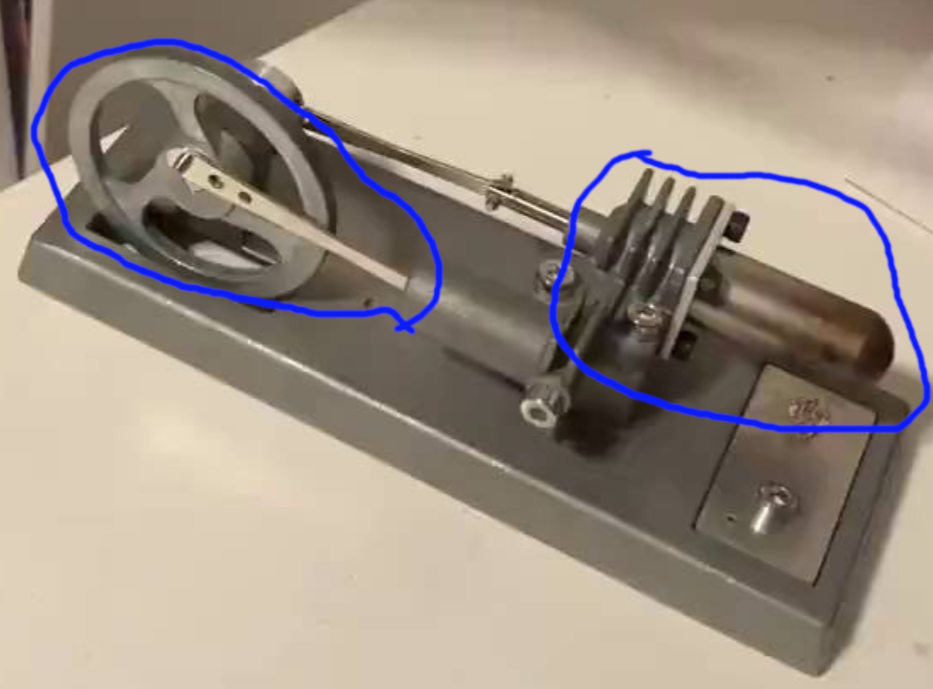
\includegraphics[width=7cm]{figures/stirling/full.png}
  \caption{A stirling engine with two sub-assemblies highlighted
  }\label{fig:stirling_full}
\end{figure}

Figure~\ref{fig:erector} shows how a model motorcycle can be broken up into
three sub-assemblies.
The Stirling engine has a single large base, but the motorcycle is simply
assembled from small pieces. Therefore, assembling the motorcycle would require
an additional set of steps at the end, to connect the sub-assemblies together.

\begin{figure}
  \begin{subfigure}{\textwidth}
    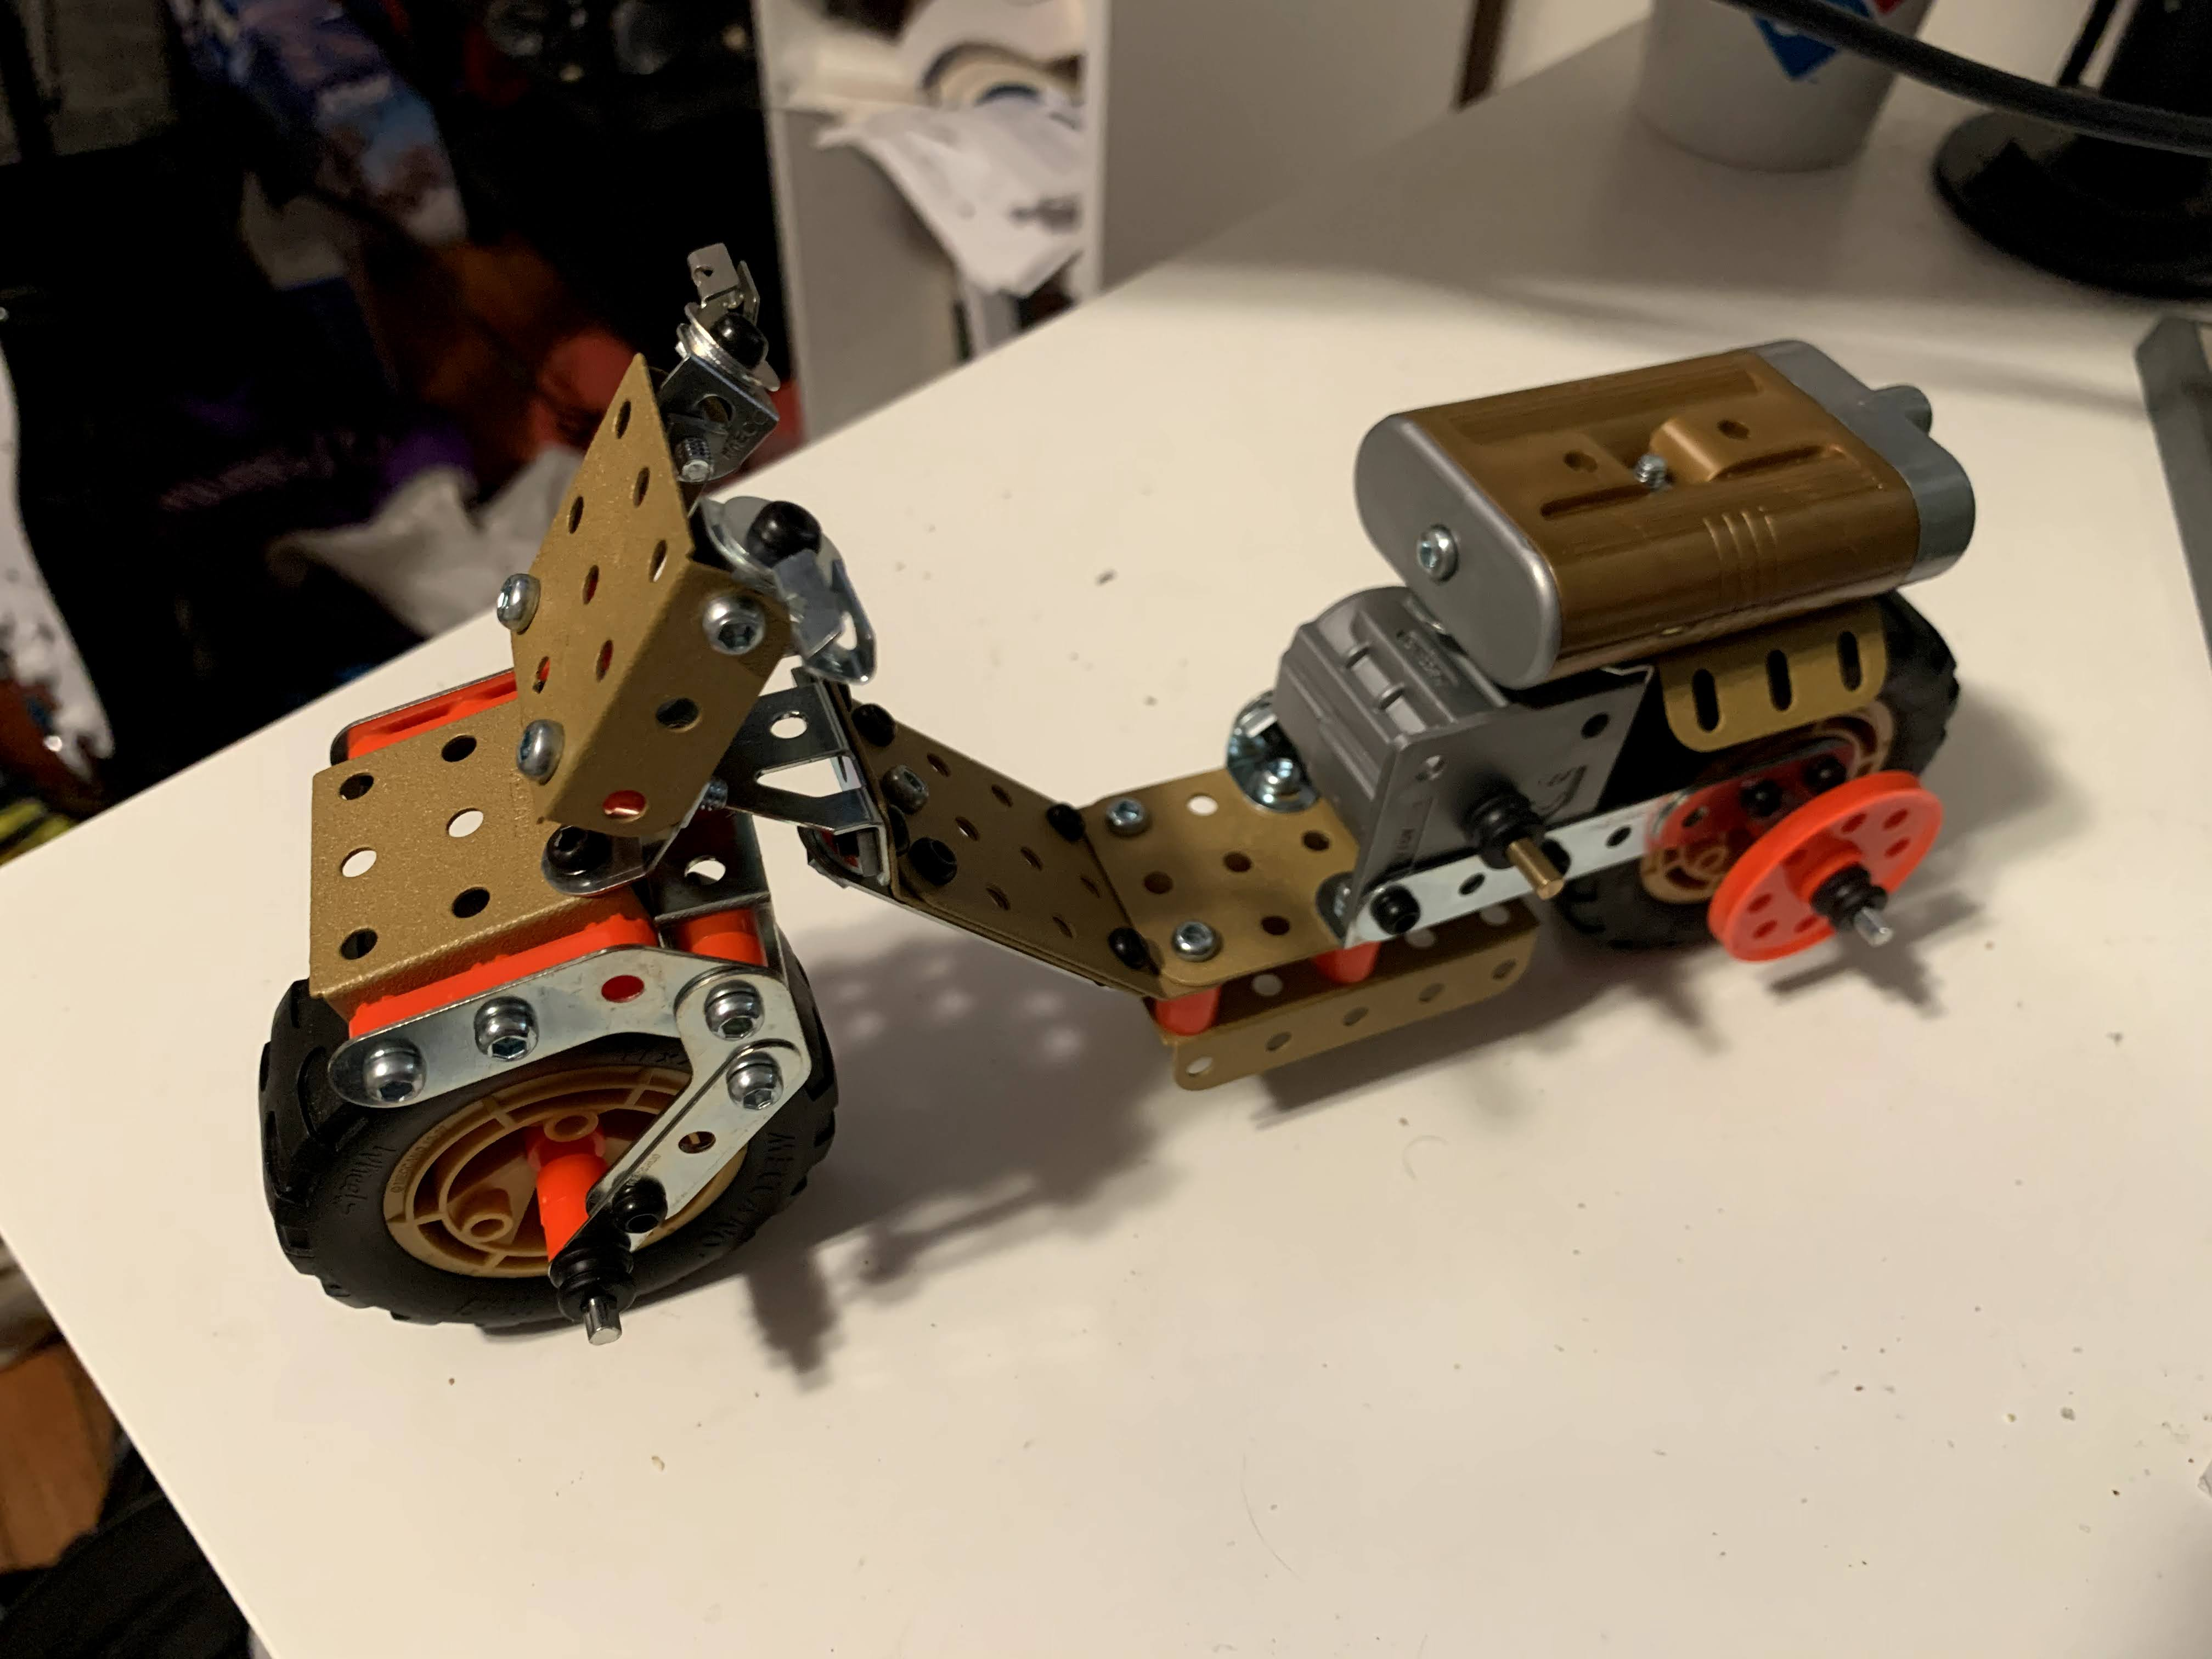
\includegraphics[width=5cm]{figures/erector/full.jpg}
    \caption{The fully-assembled model}
  \end{subfigure}
  \begin{subfigure}{\textwidth}
    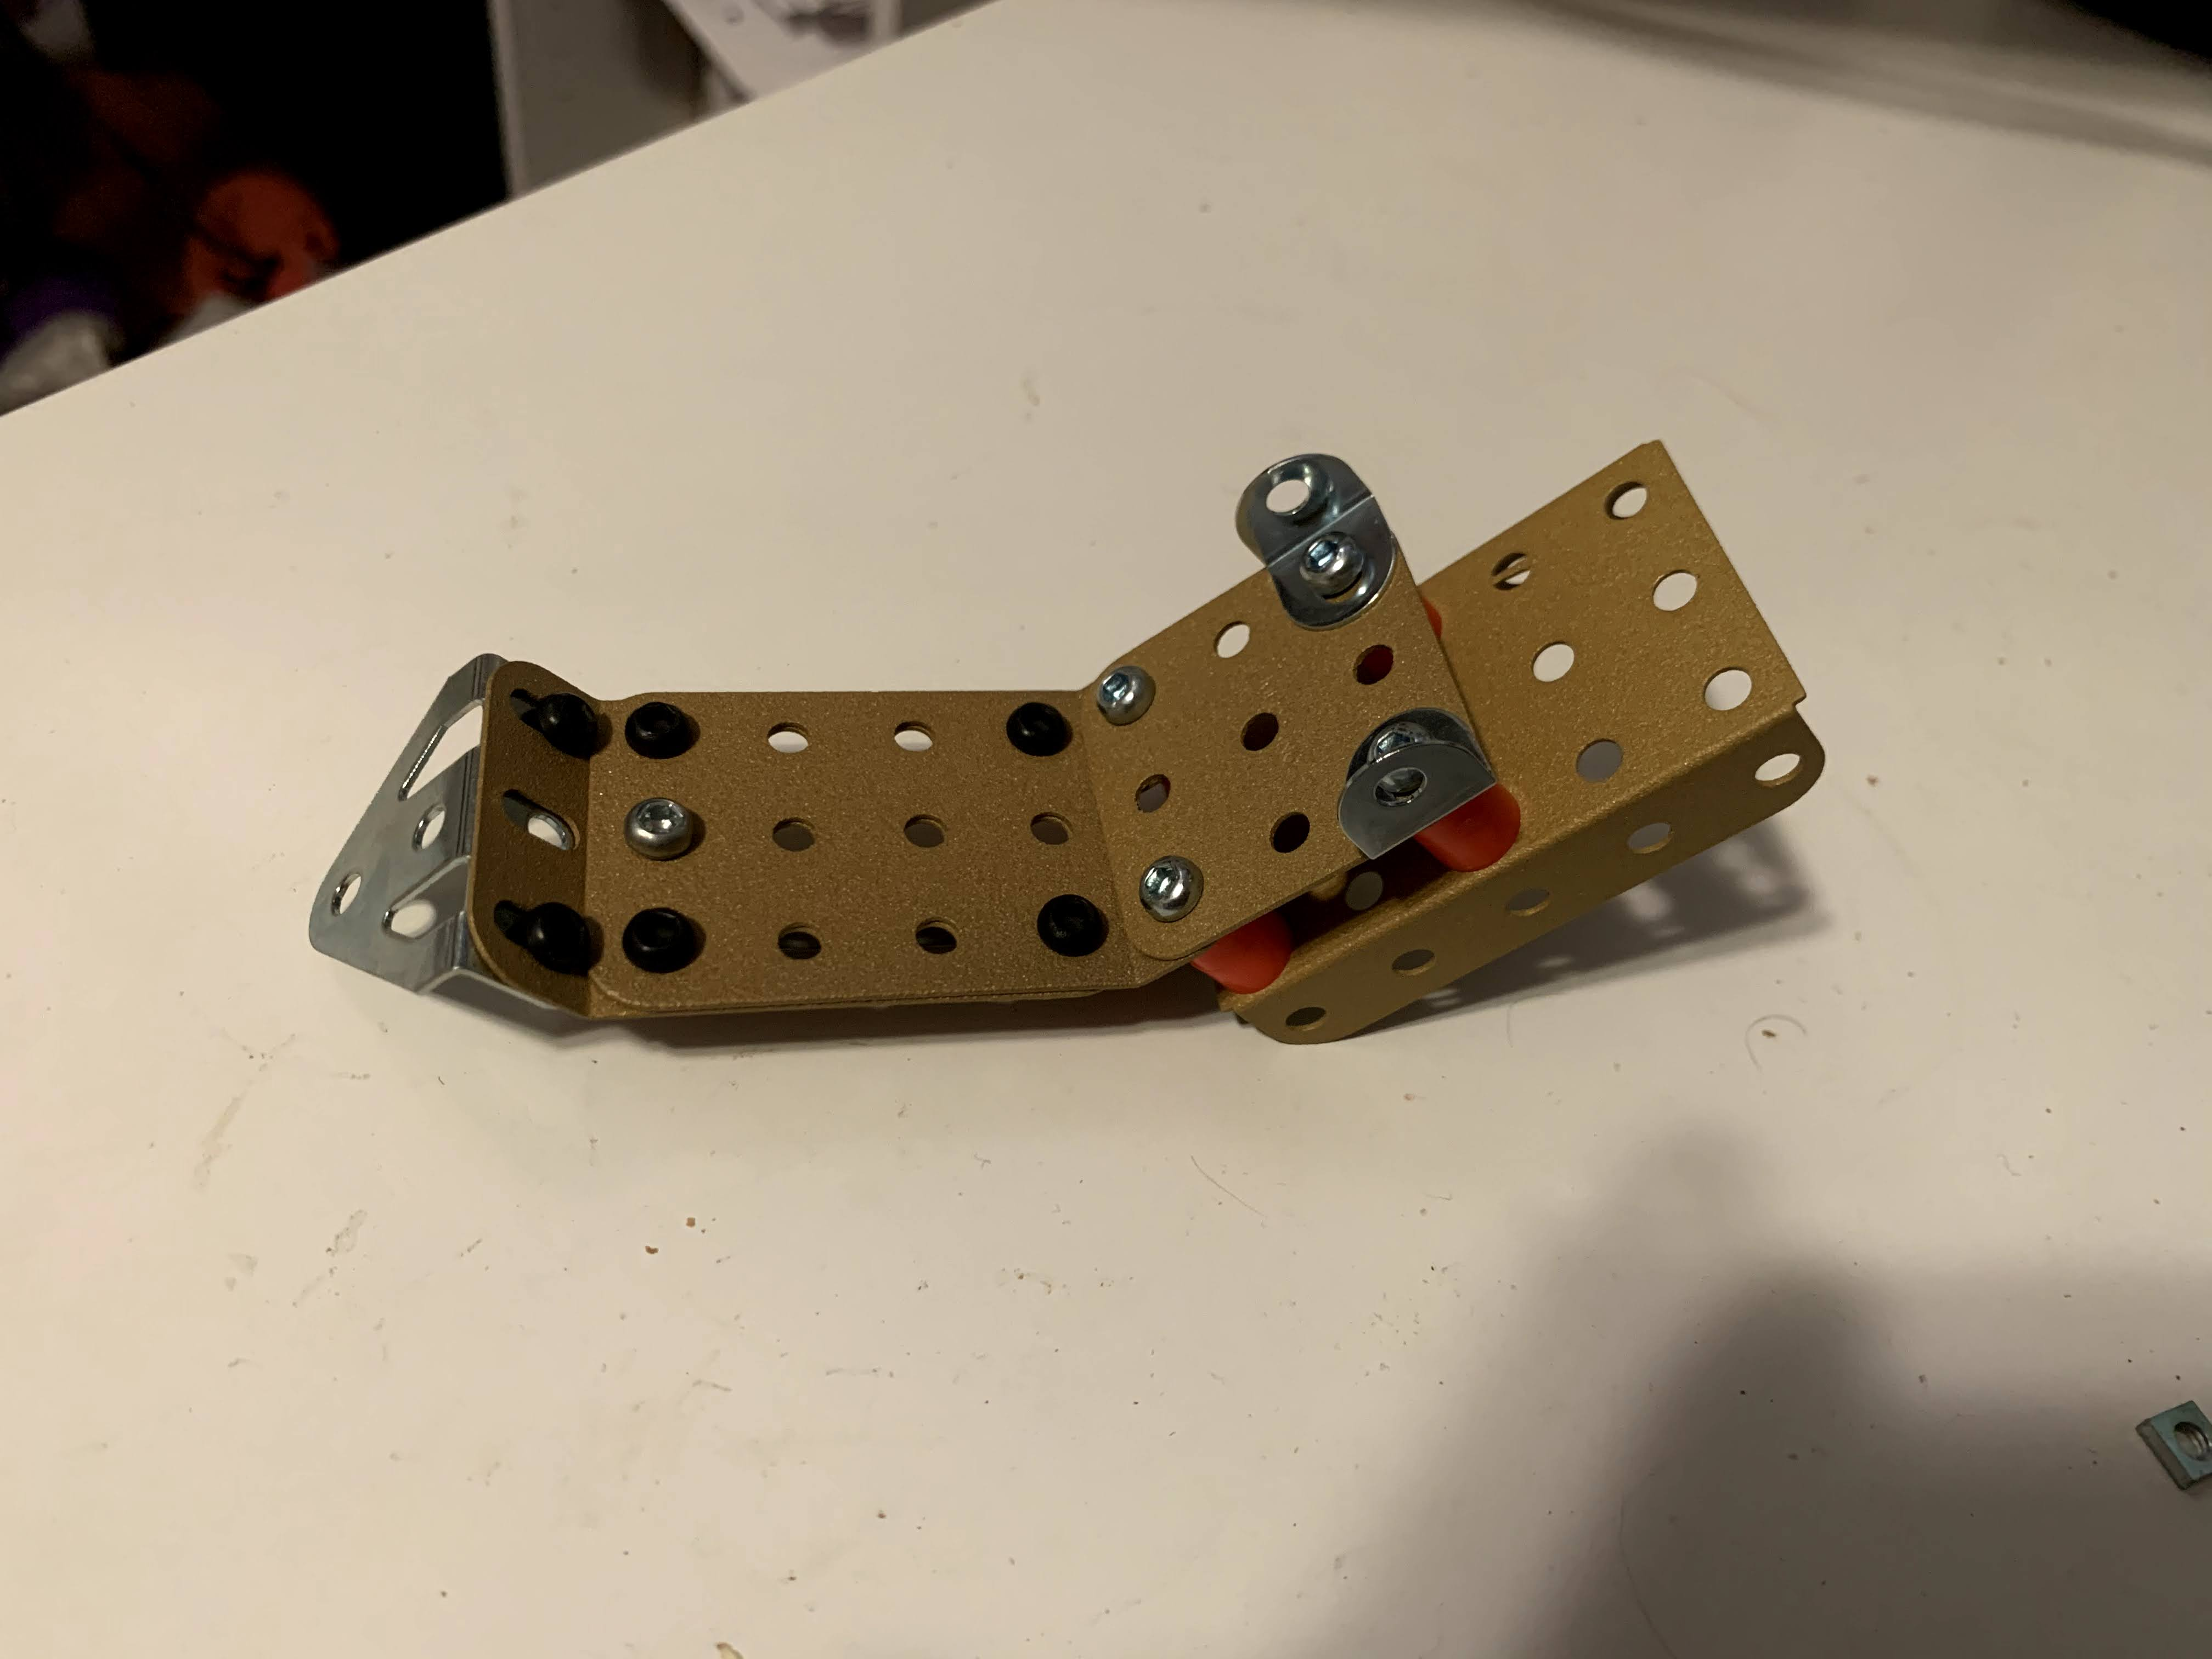
\includegraphics[width=5cm]{figures/erector/sub1.jpg}
    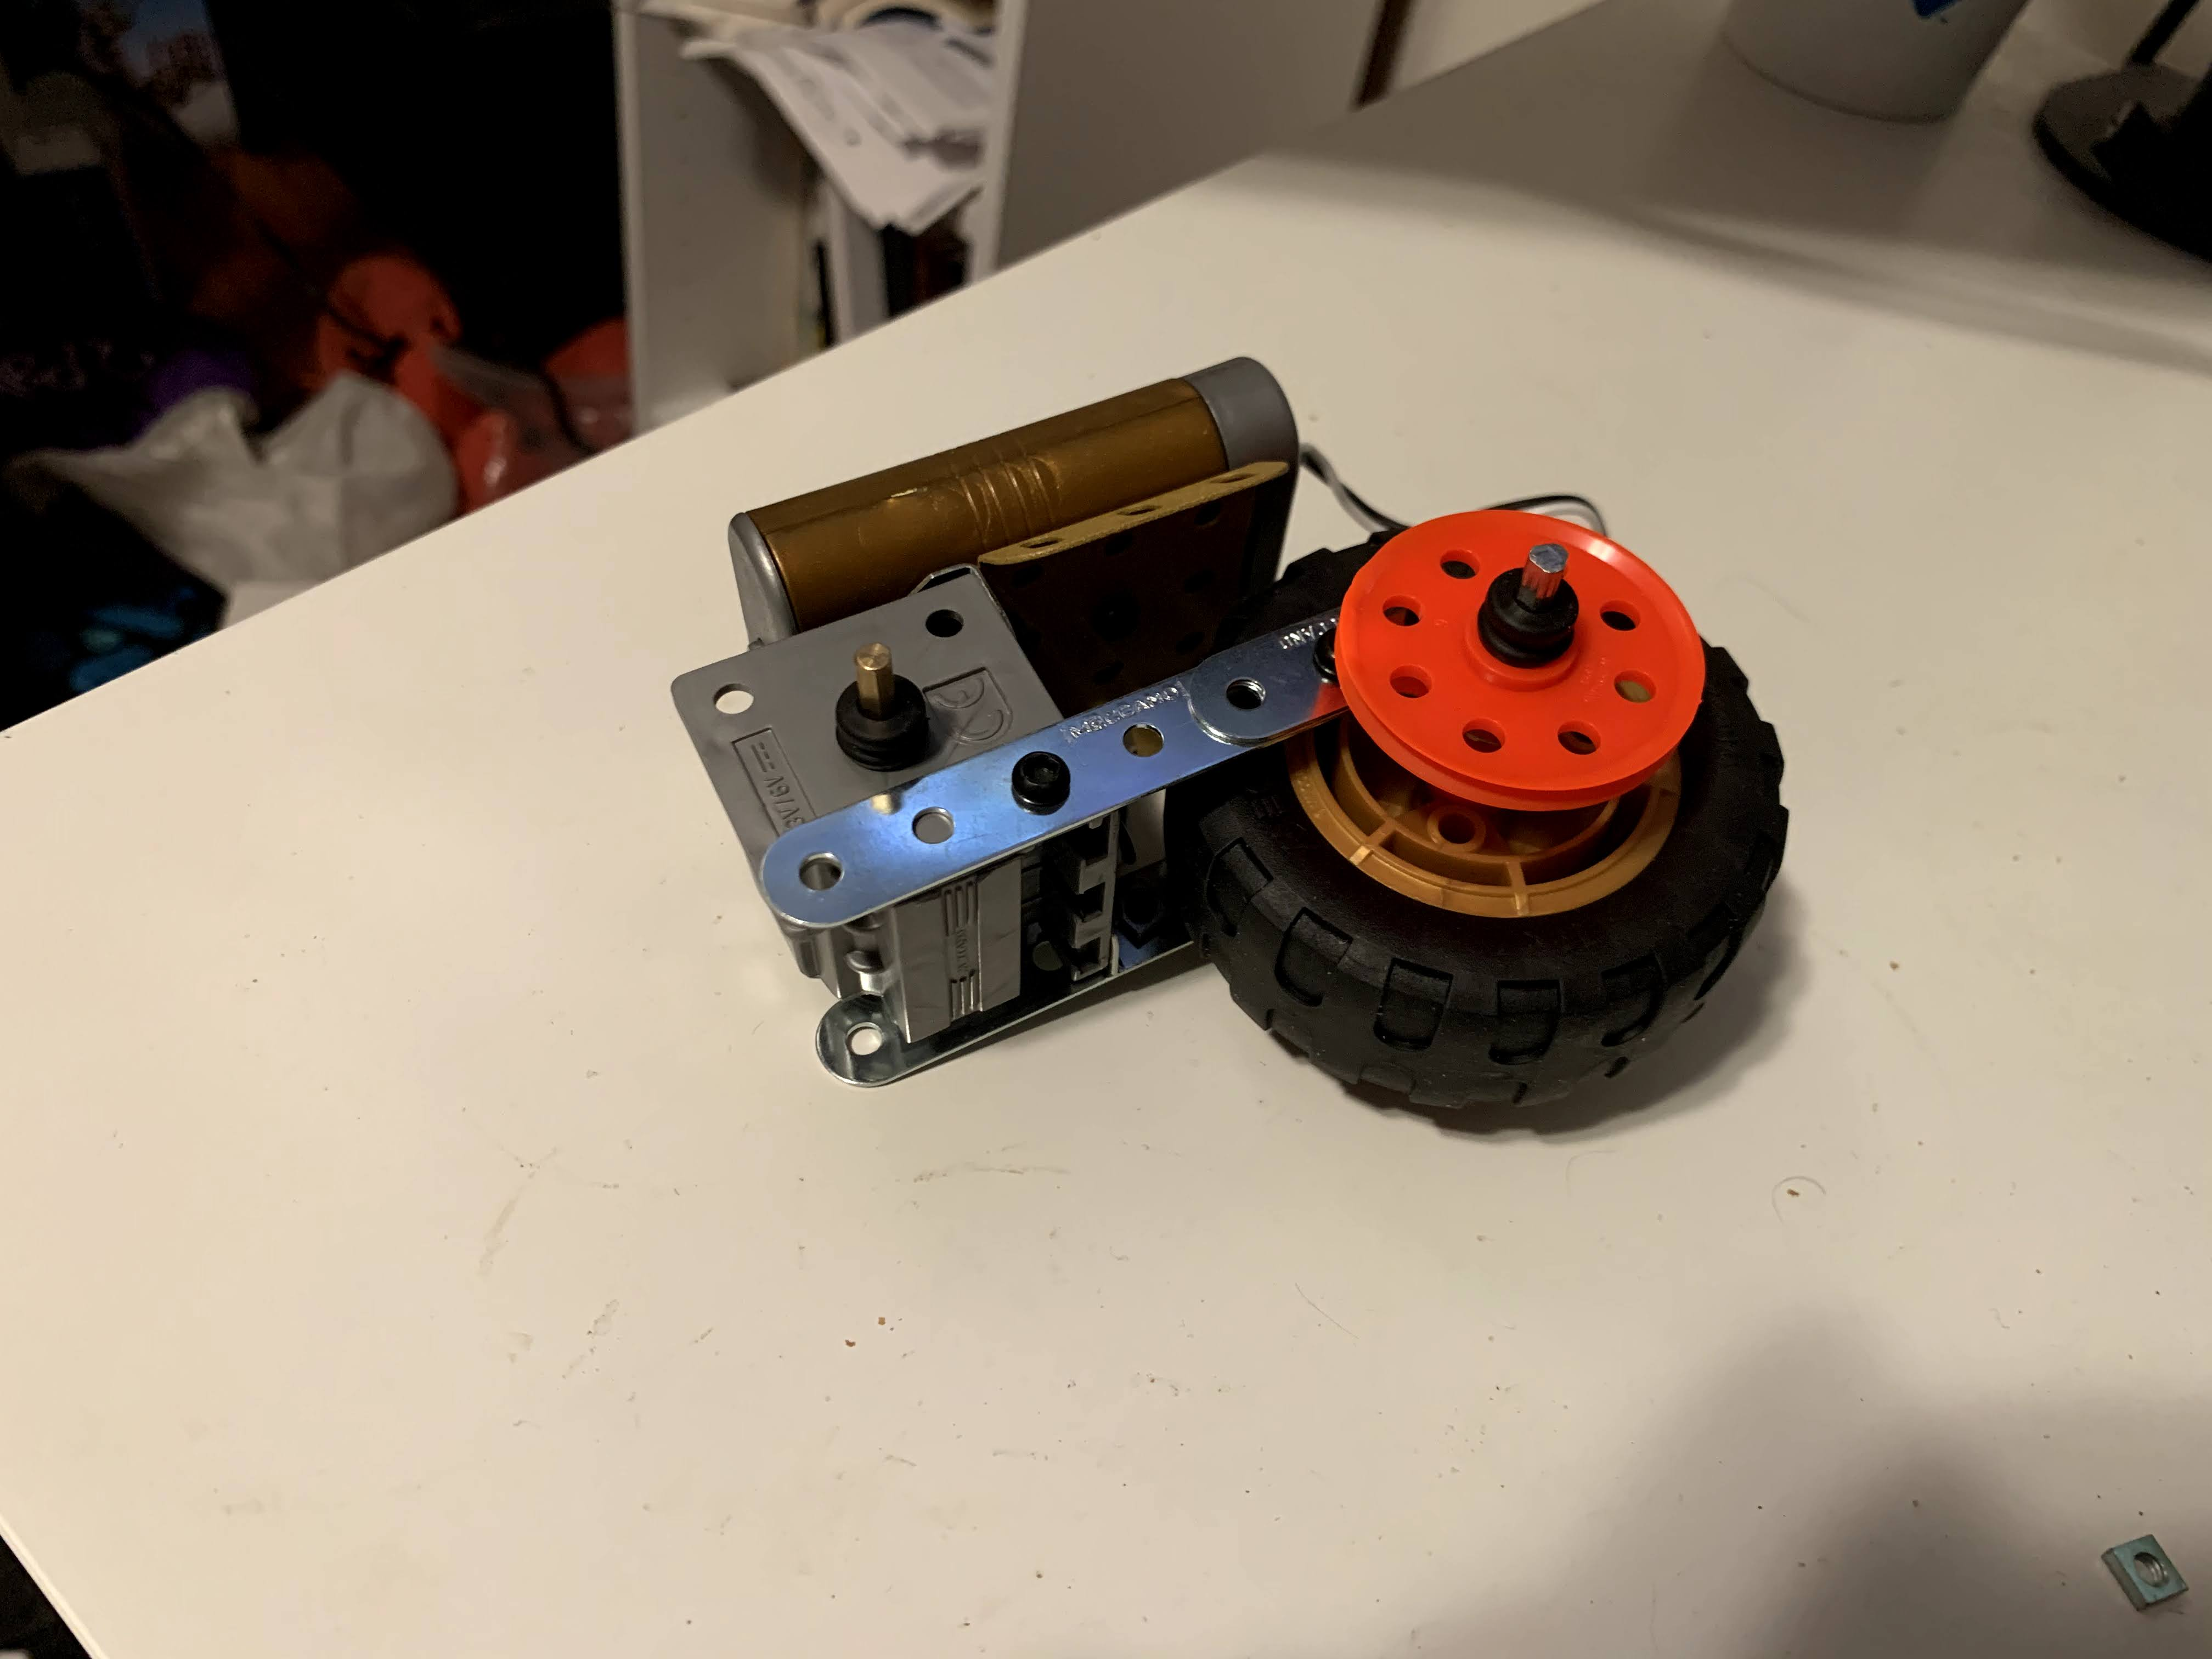
\includegraphics[width=5cm]{figures/erector/sub2.jpg}
    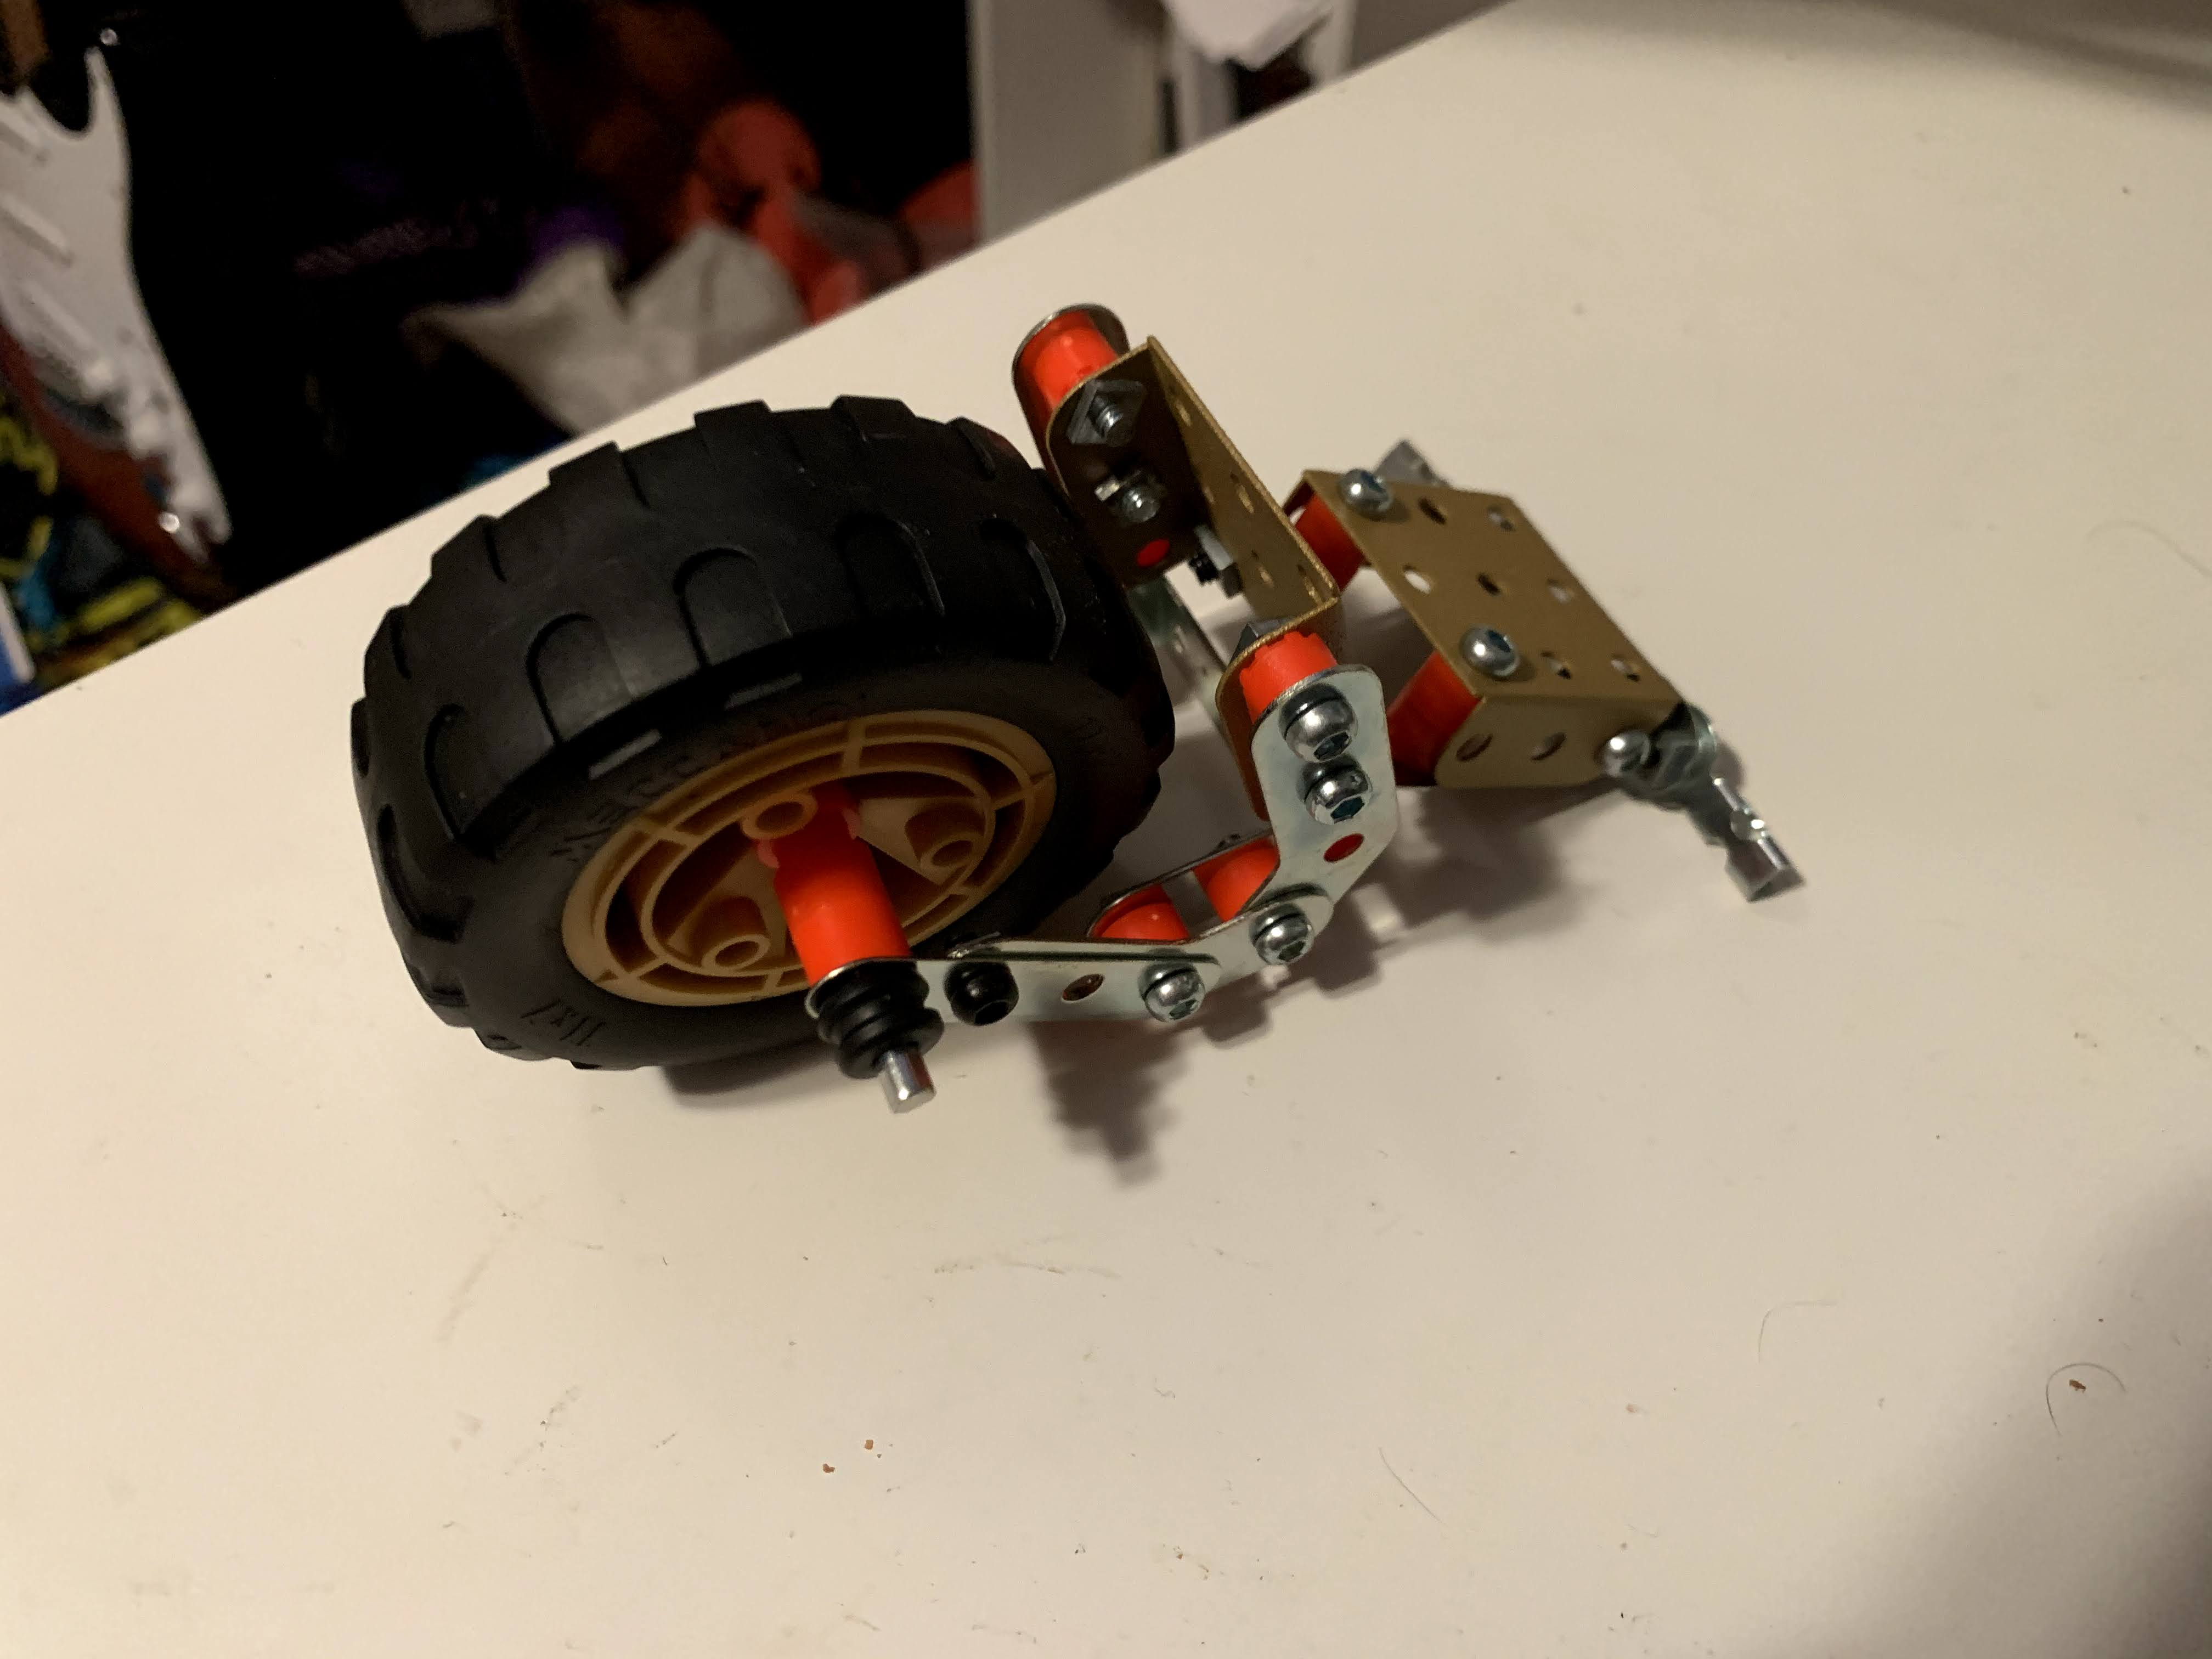
\includegraphics[width=5cm]{figures/erector/sub3.jpg}
    \caption{Sub-assemblies}
  \end{subfigure}
  \caption{A model motorcycle from a Meccano Erector kit
  }\label{fig:erector}
\end{figure}

\subsection{Implementation}

Our applications accomplish hierarchical decomposition by processing camera
images using a two stage process inspired by \citet{gebru2017finegrained}.
The first stage involves finding the region of the
image that contains the subassembly that a user is working on, using Faster
R-CNN~\cite{frcnn}.
Next, the image is cropped around this region, and the cropped region is
classified using Fast MPN-COV~\cite{Li_2018_CVPR}.
There is one Fast MPN-COV per subassembly.
The Fast MPN-COV model has one label for each step of the task that is part of
this model's subassembly.
The classification result therefore indicates the step of the task that is shown
in an image.
The application considers a step to be complete when an image from the camera
feed is classified as the label corresponding to the next step.
The architecture for this application is shown in Figure~\ref{fig:arch}.

\begin{figure}
  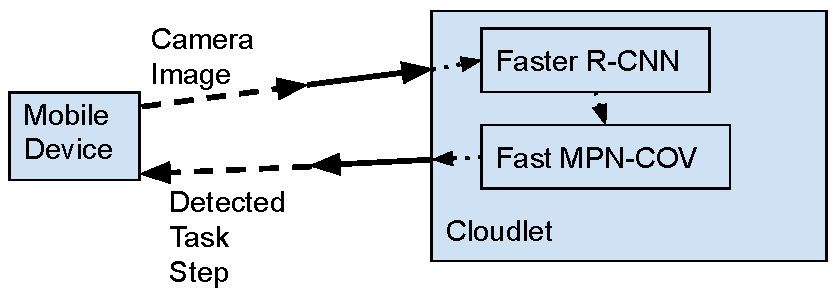
\includegraphics[width=\columnwidth]{figures/architecture.pdf}
  \caption{
    The architecture of our WCA application for the Meccano erector kit.
    The dashed lines represent a Wi-Fi connection.
    The solid lines represent a connection over Gigabit Lan.
    The dotted lines represent data transmission between components on a single
    cloudlet.
  }\label{fig:arch}
\end{figure}

\subsubsection{Error Correction}

Developers can train fine-grained classifiers to recognize specific mistakes
that a user of a WCA application might make when trying to complete a task.
An error state requires training data, the same way other steps of the task do.
When a frame gets classified as depicting an error state, the user is given
instructions about how to correct this.
Section~\ref{chap:escalation} provides further discussion about handling errors
with WCA applications.

\subsubsection{Development Tools}

We expanded the Ajalon tools~\cite{pham2021ajalon} to support hierarchical
decomposition.
Ajalon previously only supported a single object detector, which was sufficient
for toy examples such as the sandwich described in~\cite{chen2017}.
However, more complex assembly task require the use of multiple object detectors
and multiple fine-grained image classifiers.
Our improvements to Ajalon allow developers to have the application use
different computer vision models as a user progresses through a task.
This results in a single application that will automatically start
giving users instructions for the next sub-assembly after they have completed
the previous one.

\section{Our Applications}

To validate our approach, We developed WCA applications for three real assembly
tasks.
We trained models for these applications using real videos that were recorded
using a smartphone.
We manually annotated the videos with bounding boxes using CVAT.

\subsubsection{Stirling Engine}\label{sec:stirling}

This WCA application guides users through disassembling a
Stirling engine.
We have posted a video~\cite{stirling_youtube} of this application and released
the artifacts required to run it~\cite{stirling_github}.
This task requires 22 steps. All of the parts are made out of
metal, with the exception of one ring that is made out of silicone. Some steps
just require removing a single screw, and the engine looks very similar before
and after this step has been completed.

We initially ran into an issue where one of the models would misclassify a step
involving small black screws.
We fixed this by illuminating the engine with a lamp while capturing images for
training and using the application.

\subsection{Ikea Cart}

Our next application provides guidance for users assembling an Ikea Raskog
utility cart.
As with the Stirling engine, we have posted a video~\cite{ikea_youtube} of this
application and the artifacts required to run it~\cite{ikea_github}.

The task requires twenty steps to complete successfully.
However, the cart has two pairs of identical components that must be
assembled the same way.
Therefore, four of the steps are repeats of earlier steps.
The application uses the same label in cases where steps are identical.
Thus there were 16 labels, that each corresponded to the 16 unique steps.
In addition, we developed the application to detect one error state, so there
were 17 possible labels that our models could output.
We split the task into three subassemblies.
The subassemblies and task steps are shown in figure~\ref{fig:ikea_cart}.

The repeated steps are repeated in pairs. For example, step 1 is performed,
followed by step 2.
Then both are repeated.
Repeating steps in pairs avoids the situation where two consecutive steps
correspond to the same label from the classifier.

\begin{figure}
  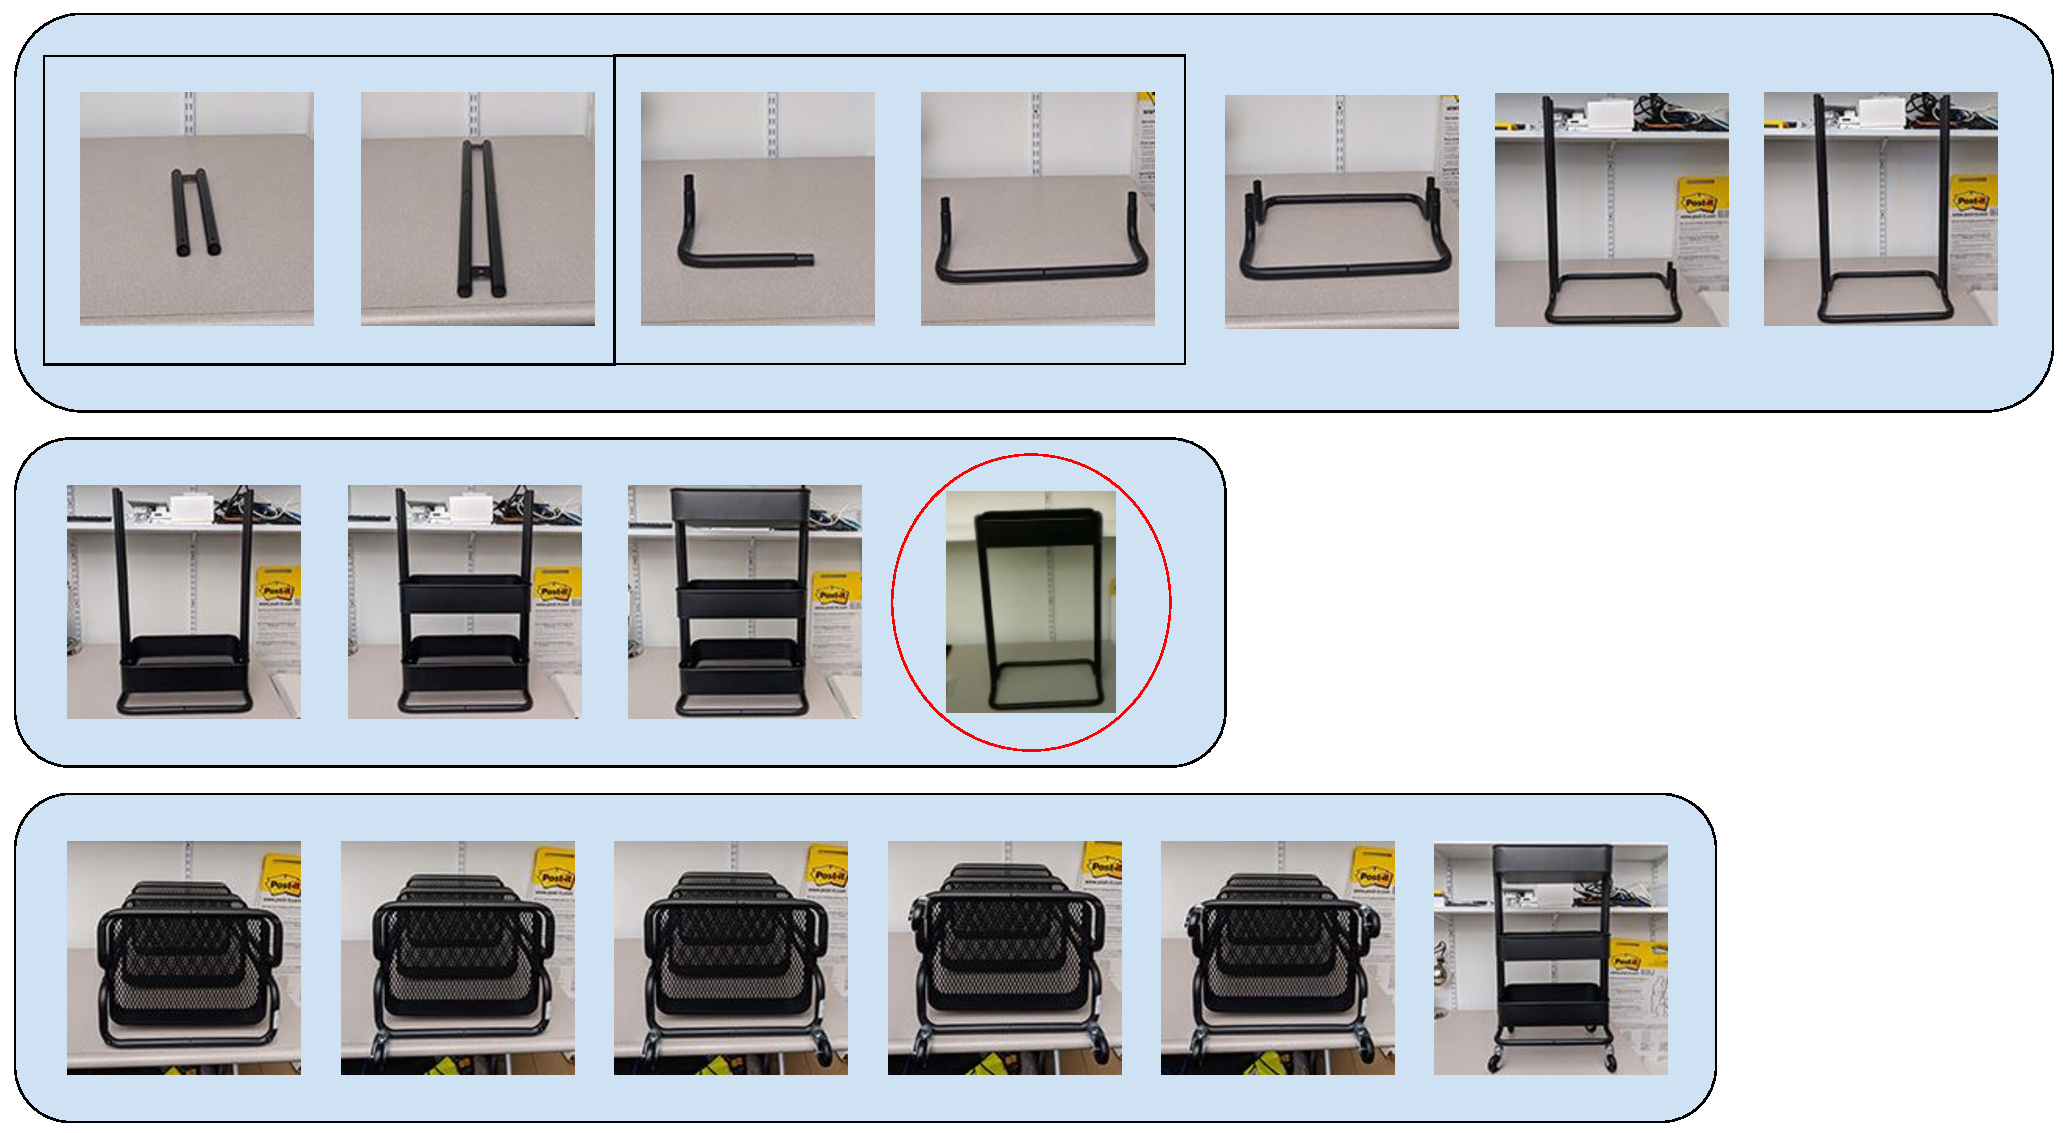
\includegraphics[width=\columnwidth]{figures/ikea_subassemblies.pdf}
  \caption{
    The steps detected by our Ikea WCA application.
    The blue rectangles with rounded corners represent subassemblies.
    The steps in the rectangles without rounded corners are repeated.
    The error state appears in the red circle.
  }\label{fig:ikea_cart}
\end{figure}

\section{Implementation Details}

We captured images at 1920x1080 pixels, and transmitted these to the cloudlet at
their full resolution.
This is the highest resolution that Android CameraX's ImageAnalysis use case
supports.
After processing the images with Faster R-CNN, the application crops them around
the region that likely contains the object.
The cropped image is resized to 448x448 pixels and then classified by Fast
MPN-COV.
By starting with a large initial image, we ensured that the cropped image would
be at least 448x448 pixels.

We also saw an improvement in performance after removing images that had the
same perceptual hash value from our train, validation, and test sets. We made
sure that all images (across all three sets) had unique perceptual hash values.

\subsection{Realtime Data}

The code for many computer vision models are written to run inference on batches
of images that are stored on disk. The torchvision package contains functions
for loading images from disk, in batches. Using these models in WCA applications
requires modifying the code to run the models on images being transmitted over
the network, one by one. The input batch size must be set to 1, because anything
larger would require building up a queue of images that would be run through the
model together as a single input. A larger batch size would improve the
frame rate for inference, but hurt the latency.

Live data must be as similar as possible to the data that the models are trained
on. For example, converting a
JPEG image to raw pixel values using OpenCV will result in slightly different
values than using Pillow will. We observed that our Fast MPN-COV model performed
significantly better with images opened using Pillow than with images opened
using OpenCV. The training images were opened using Pillow, but we did not
expect opening JPEGs with OpenCV and Pillow to result in different color values.

Processing images while a user is in the middle of a step wastes bandwidth and
computing resources on cloudlets.
In addition, it might lead to an application mistakenly
believing that a step has been completed before it actually has been.
We experimented with a filter that requires a set of consecutive frames to have
identical perceptual hash values.
This essentially means that a certain number of images in a row all had to look
the same.
This technique worked well for WCA applications running on a smartphone mounted
to a tripod.
But it did not work well for WCA applications running on a Google Glass, due to
the motion of the user's head.
Instead, we required a sequence of sequential images to be assigned the same
label by the classifier.
This helped avoid cases where the application mistakenly believed a step had
been completed while a user was still in the middle of it.
But it did not save computing resources on the cloudlet, because every frame had
to be processed.
